%
% IT.
% Information Technology
%
% Aleph Objects Operations Manual
%
% Copyright (C) 2014, 2015 Aleph Objects, Inc.
%
% This document is licensed under the Creative Commons Attribution 4.0
% International Public License (CC BY-SA 4.0) by Aleph Objects, Inc.
%

\section{Employee Services}
These are URLs that are for Aleph Objects employee use.

\subsection{Website Analytics}
\url{https://analytics.alephobjects.com} --- Website analytics.

When website users go to various Aleph Objects websites, such as lulzbot.com,
they also pass info about the visit to the analytics server. The collected
data is not public (at present).

\begin{figure}[h!]
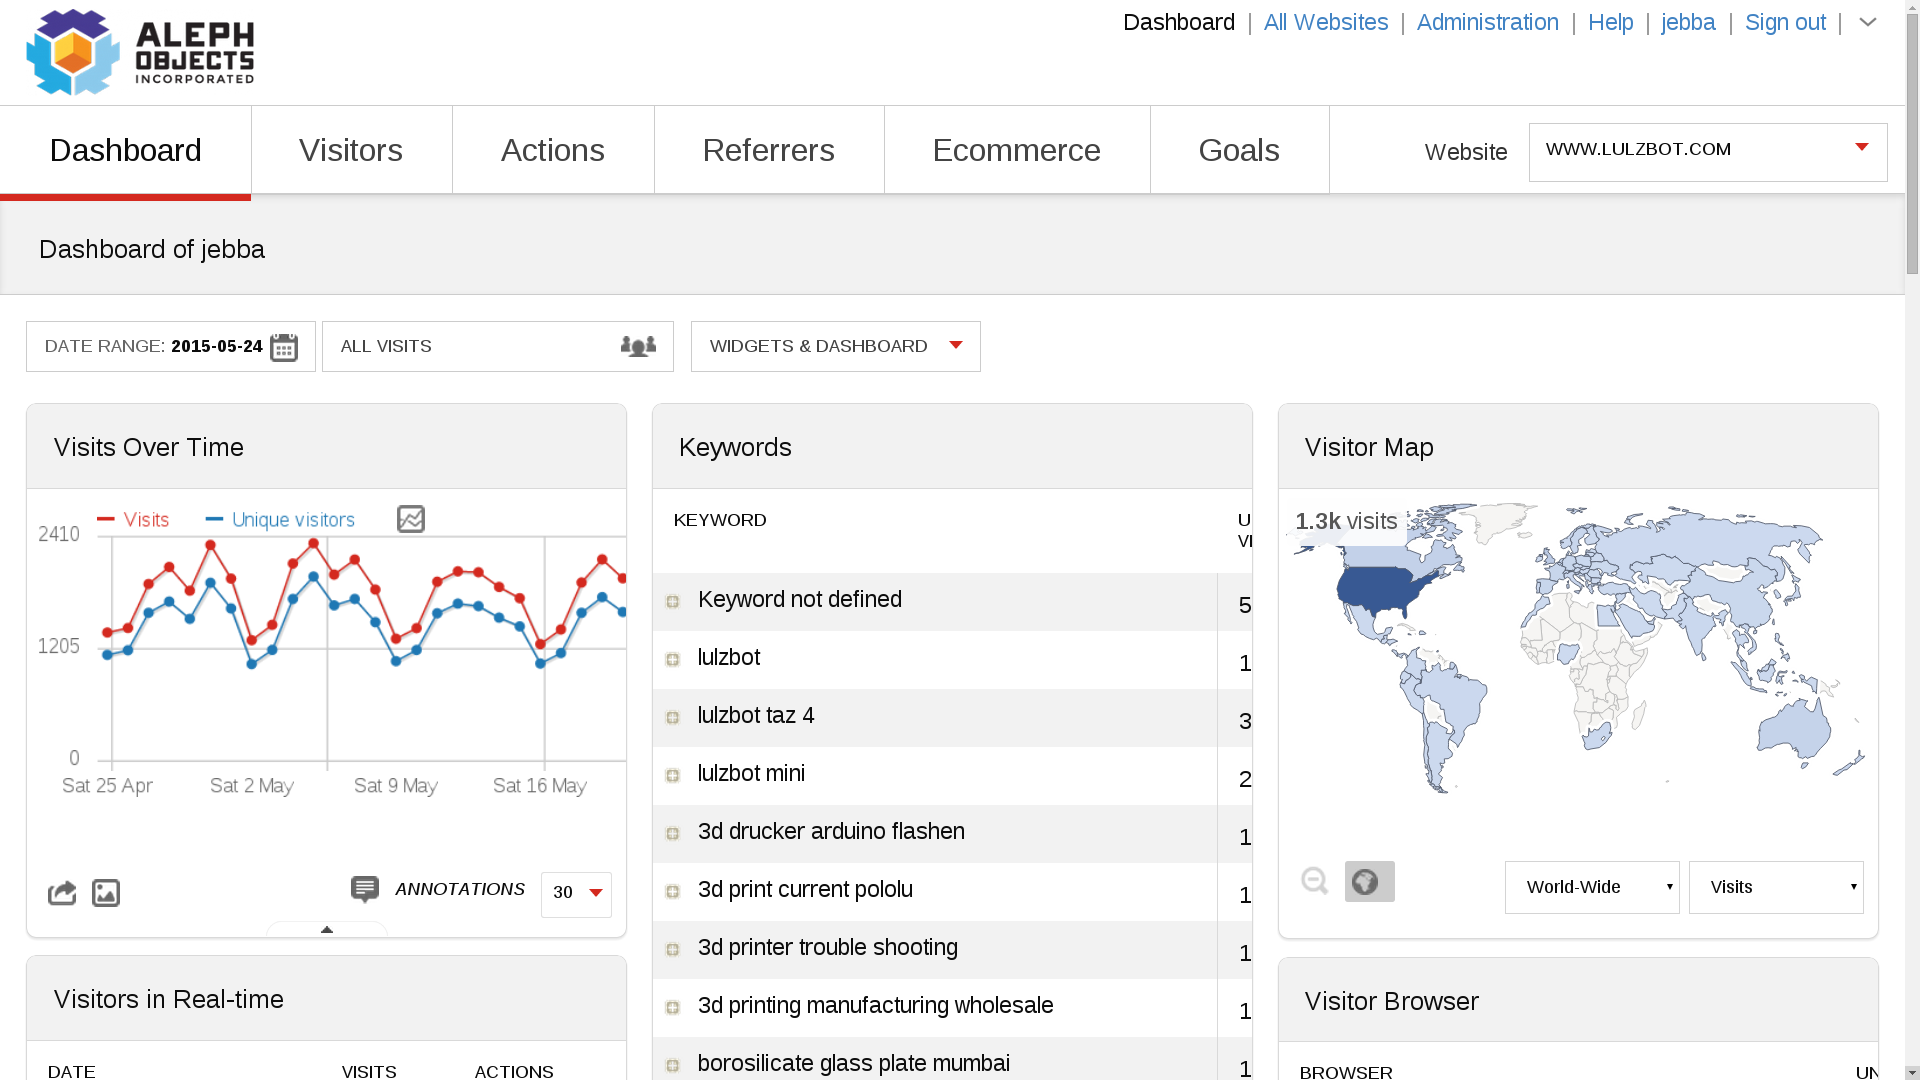
\includegraphics[keepaspectratio=true,height=1.10\textheight,width=1.00\textwidth,angle=0]{analytics.alephobjects.com.png}
 \caption{Aleph Objects analytics, \href{analytics.alephobjects.com}{analytics.alephobjects.com}}
 \label{fig:analyticsalephobjectscom}
\end{figure}

\subsection{Webmail Server}
\url{https://aomail.alephobjects.com} --- Webmail server.
\begin{figure}[h!]
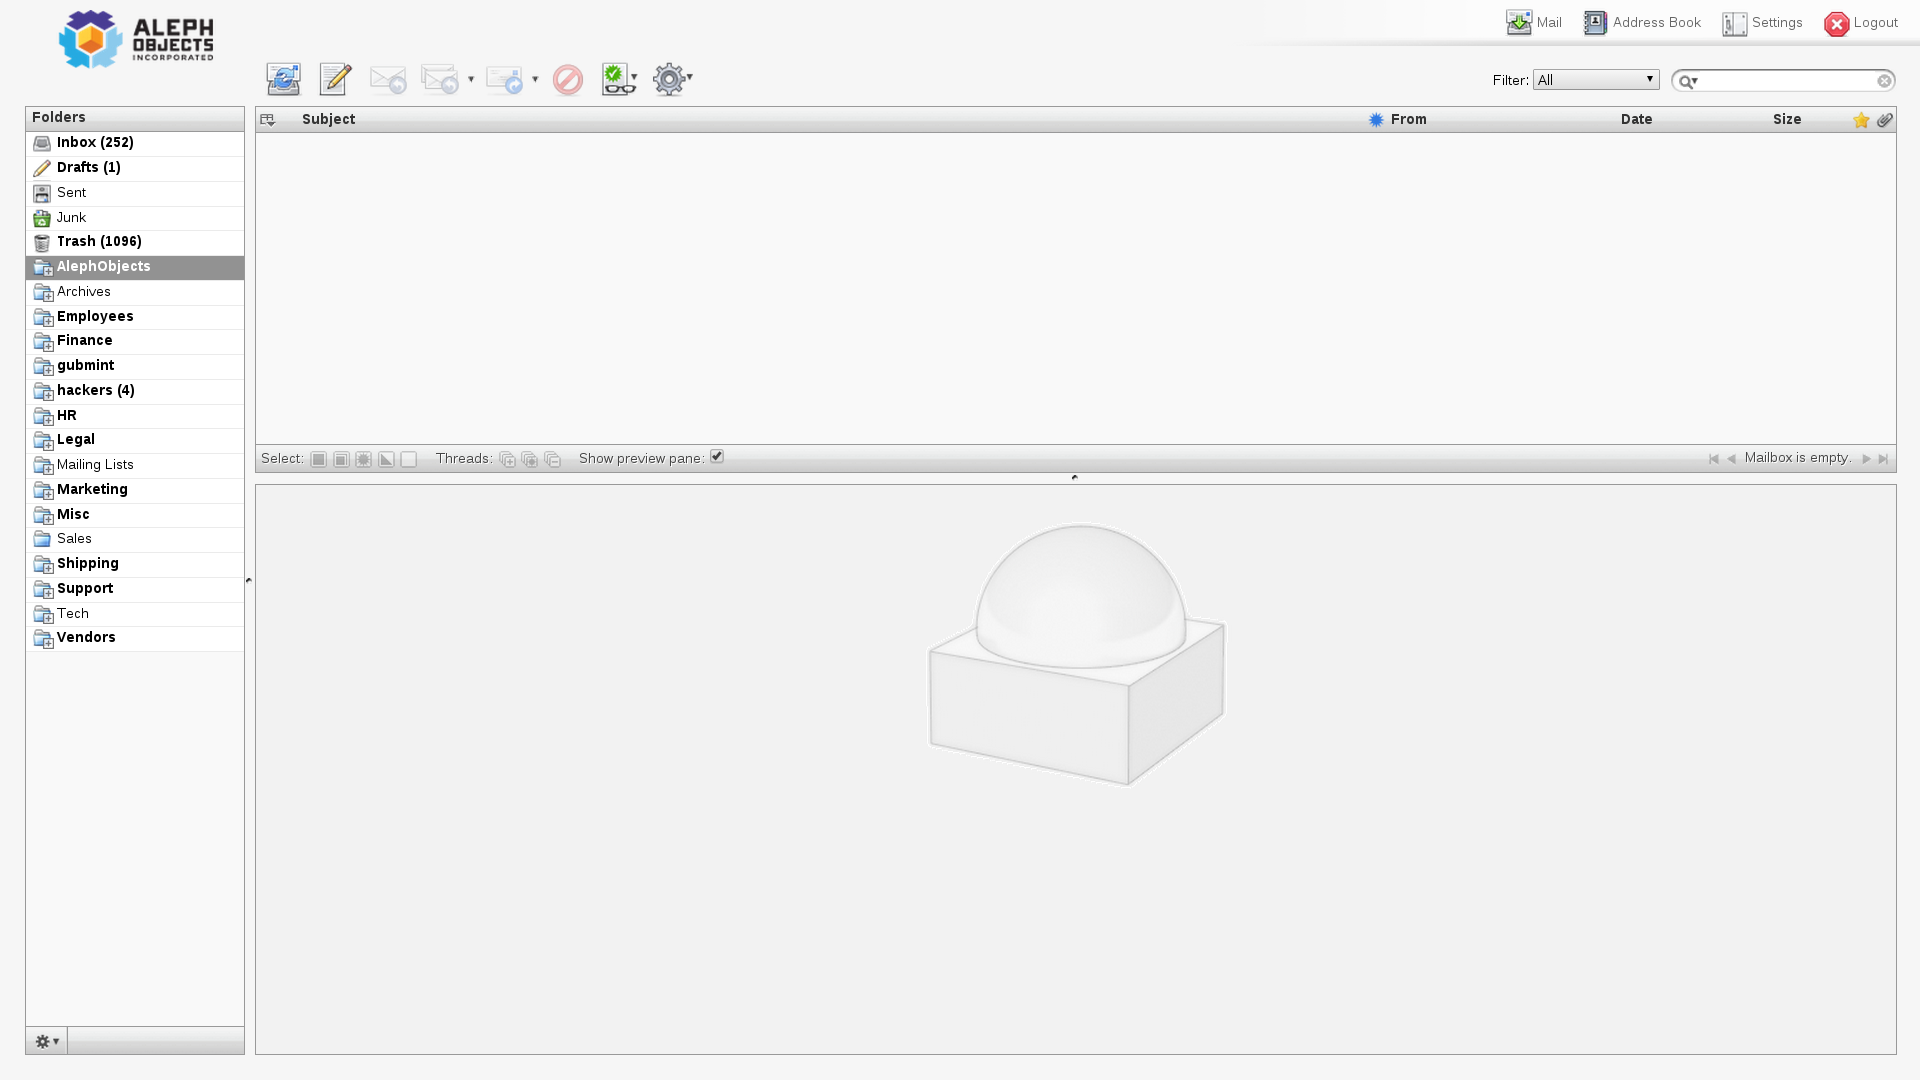
\includegraphics[keepaspectratio=true,height=1.10\textheight,width=1.00\textwidth,angle=0]{aomail.alephobjects.com.png}
 \caption{Aleph Objects Web Mail, \href{aomail.alephobjects.com}{aomail.alephobjects.com}}
 \label{fig:aomailalephobjectscom}
\end{figure}

\subsection{Backup Server}
\url{https://belly1.alephobjects.com} --- Backup server.

\subsection{ERP Server}
\url{https://erp.alephobjects.com} --- ERP server.
\begin{figure}[h!]
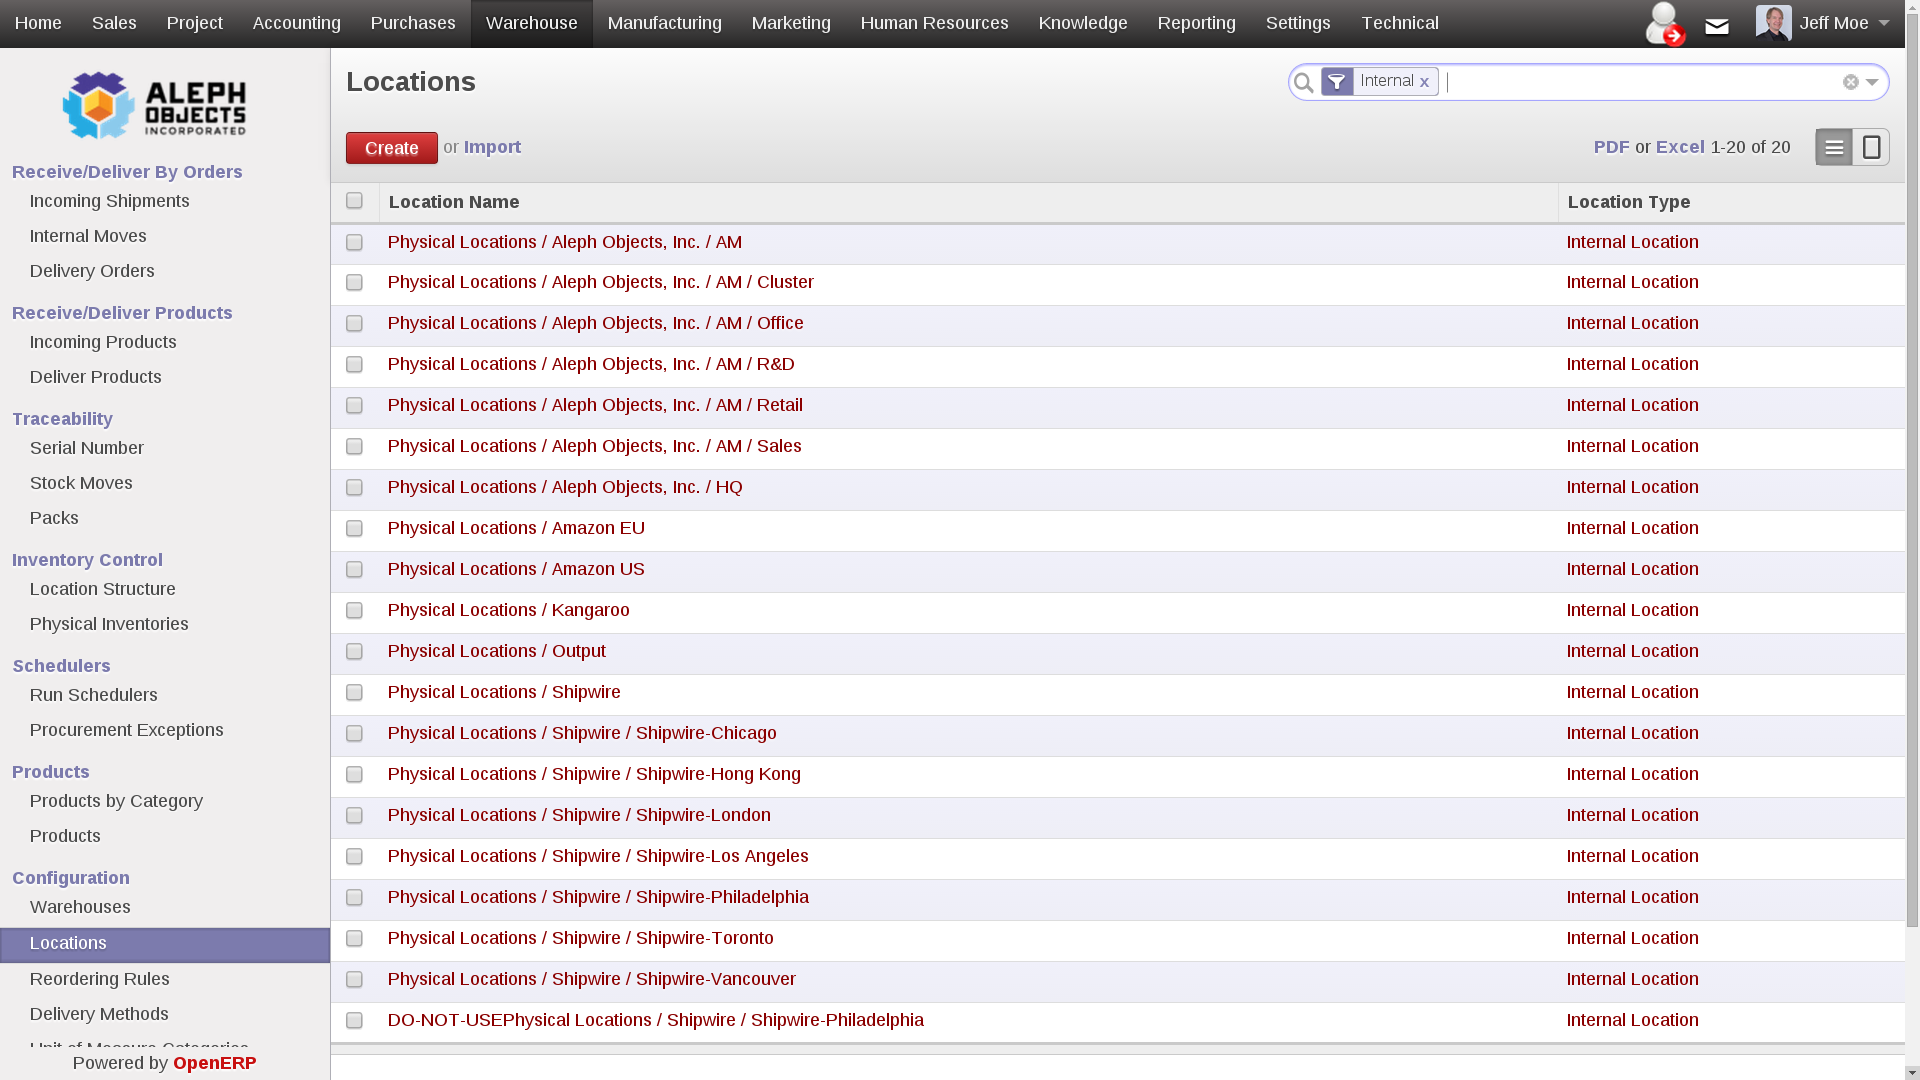
\includegraphics[keepaspectratio=true,height=1.10\textheight,width=1.00\textwidth,angle=0]{erp.alephobjects.com.png}
 \caption{Aleph Objects ERP Server, \href{erp.alephobjects.com}{erp.alephobjects.com}}
 \label{fig:erpalephobjectscom}
\end{figure}

\subsection{Network Monitoring}
\url{https://ops.alephobjects.com} --- Network monitoring.
\begin{figure}[h!]
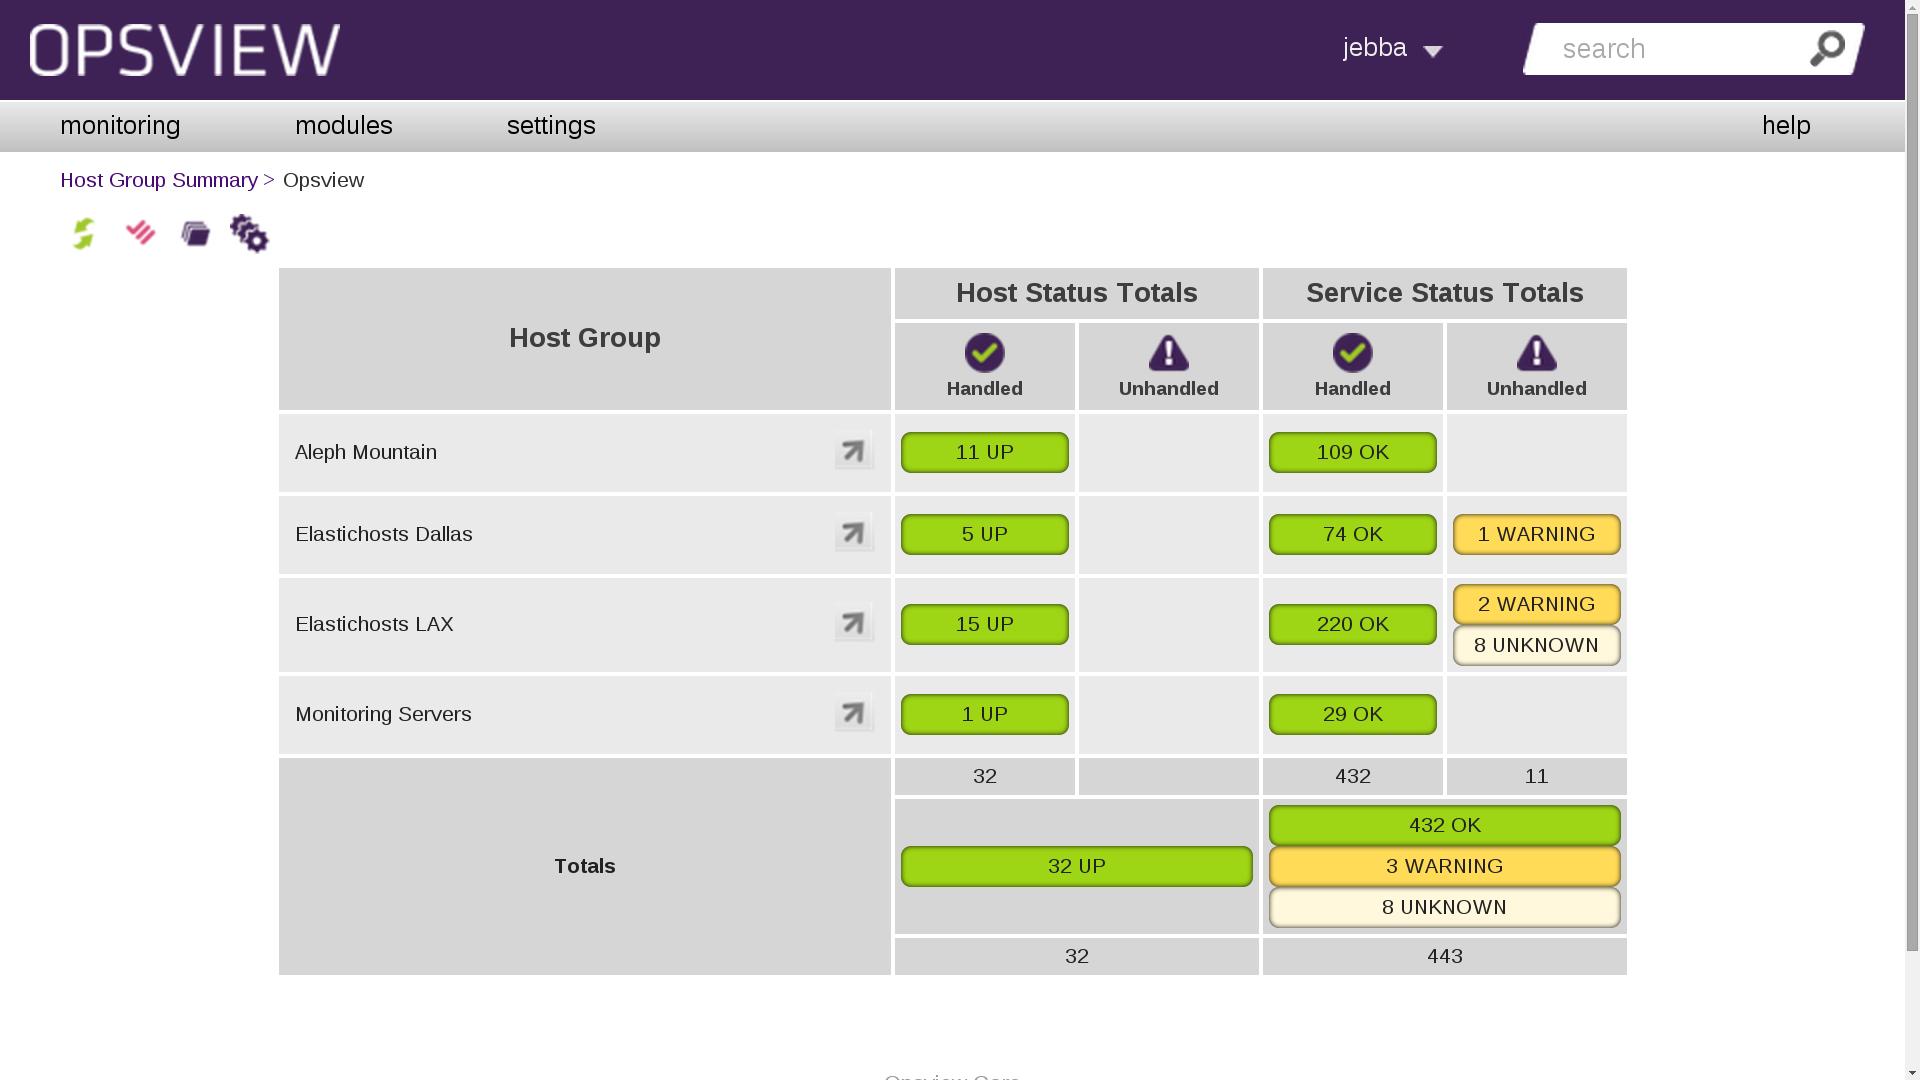
\includegraphics[keepaspectratio=true,height=1.10\textheight,width=1.00\textwidth,angle=0]{ops.alephobjects.com.png}
 \caption{Aleph Objects Opsview Monitoring, \href{ops.alephobjects.com}{ops.alephobjects.com}}
 \label{fig:opsalephobjectscom}
\end{figure}

\subsection{Project Tracking}
\url{https://projects.alephobjects.com} --- Project tracking.

This is a new system for us, it isn't heavily used (yet).

\begin{figure}[h!]
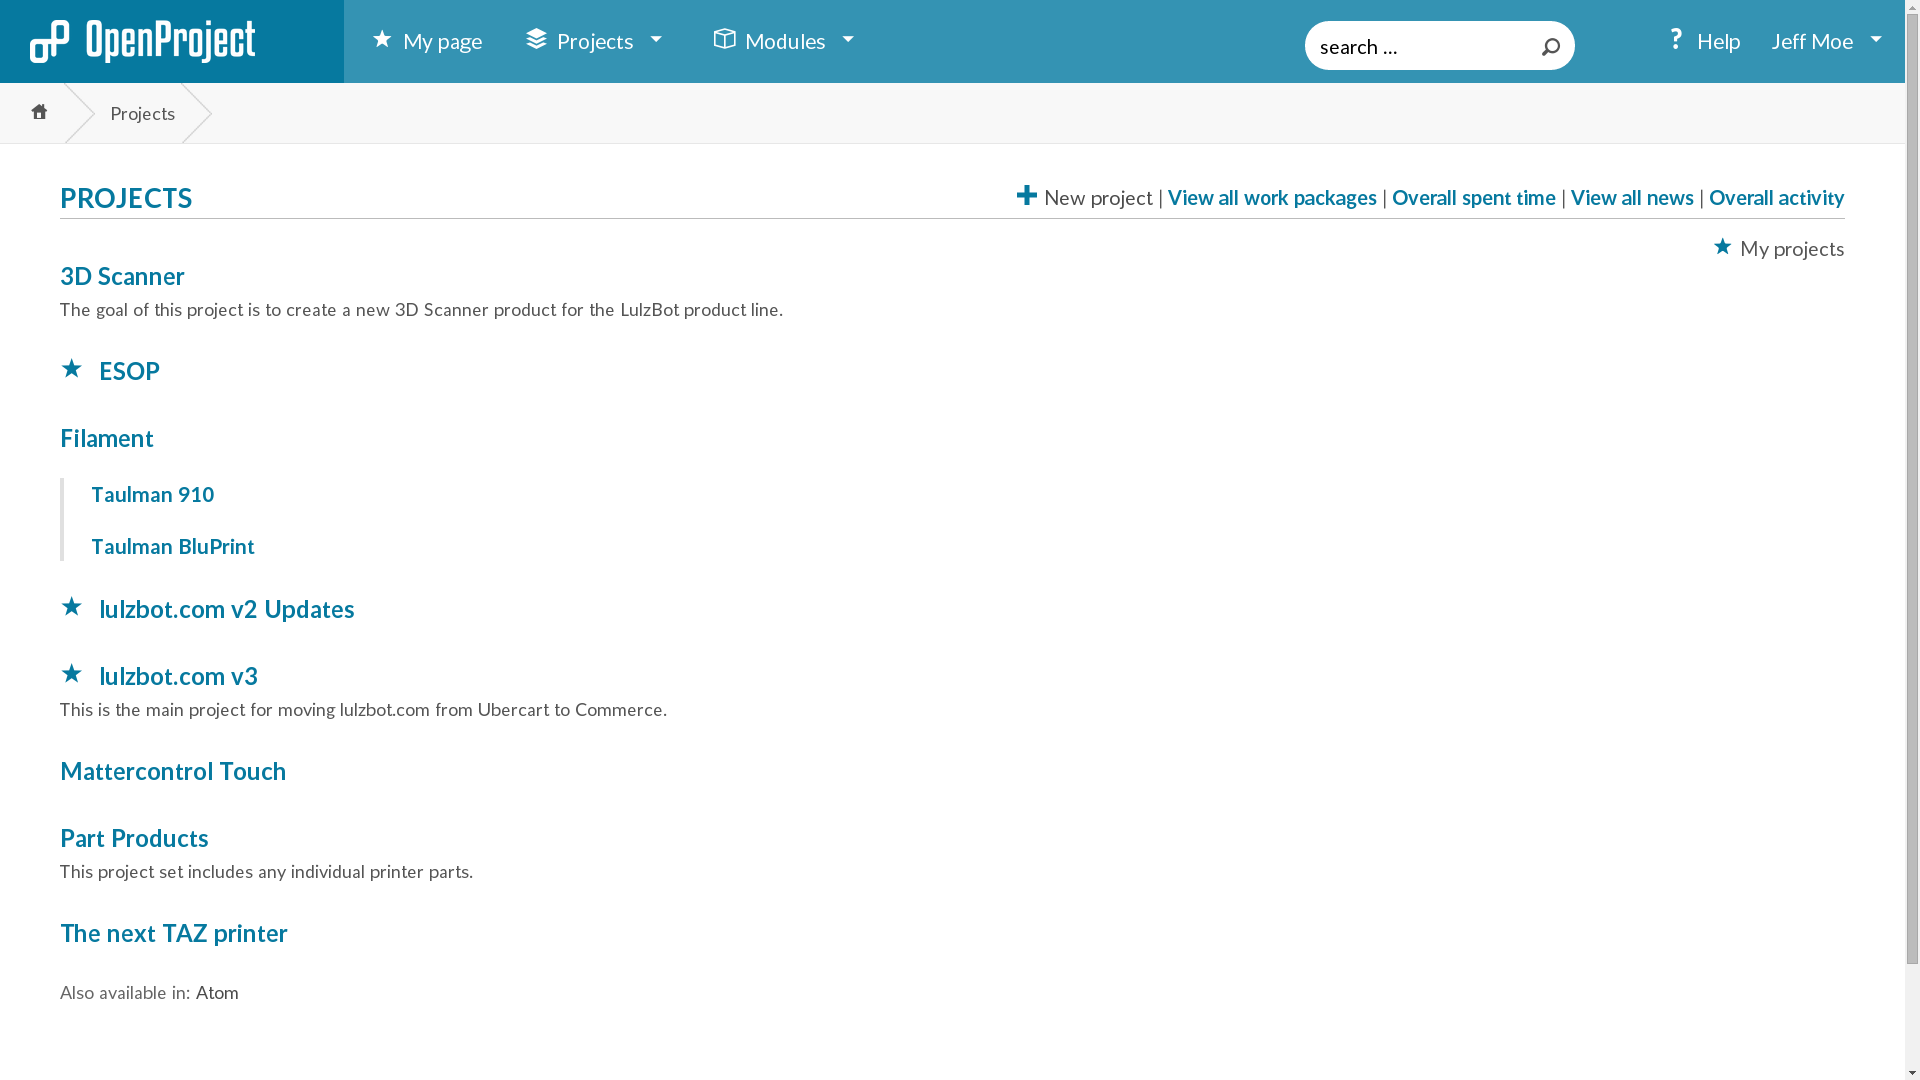
\includegraphics[keepaspectratio=true,height=1.10\textheight,width=1.00\textwidth,angle=0]{projects.alephobjects.com.png}
 \caption{Aleph Objects Project Tracking, \href{projects.alephobjects.com}{projects.alephobjects.com}}
 \label{fig:projectsalephobjectscom}
\end{figure}

\subsection{Wiki}
\url{https://wiki.alephobjects.com} --- Development wiki.

